\documentclass[10pt,a4paper]{article}
\usepackage{fontspec}
\defaultfontfeatures{Mapping=tex-text}
\usepackage{xunicode}
\usepackage{xltxtra}
%\setmainfont{???}
\usepackage{polyglossia}
\setdefaultlanguage{english}
\usepackage{amsmath}
\usepackage{amsfonts}
\usepackage{amssymb}
 \usepackage{siunitx}
\usepackage{xeCJK}
\usepackage{ctex}
\usepackage[left=2cm,right=2cm,top=2cm,bottom=2cm]{geometry}
\author{翁俊}
\title{江门中微子(JUNO)调研报告}
\begin{document}
\maketitle
\newpage
\tableofcontents
\newpage

\section{JUNO实验课题背景与研究目标} \label{overview}%------------------------------
江门中微子实验是是继大亚湾反应堆中微子实验之后由中国主持的第二个大型中微子实验。实验站将建在地下700米深处,实验计划最早在2021年投入运行并开始物理取数,运行至少20年。实验建造的中微子探测器将是世界上能量精度最高、规模最大的液体闪烁体探测器。这一实验的启动标志着我国中微子实验研究从起步到跨越的转变。
\subsection{神奇的幽灵粒子}\label{sub:sysover}
中微子又译作微中子,是轻子)的一种,是组成自然界的最基本的粒子之一,常用符号ν表示。中微子不带电,自旋为1/2,质量非常轻(有的小于电子的百万分之一),以接近光速运动。

粒子物理的研究结果表明,构成物质世界的最基本的粒子有12种,包括6种夸克,3种带电轻子(电子,$\nu$子和$\tau$子)和3种中微子(电子中微子,$\nu$中微子和$\tau$中微子)。

\begin{figure}[ht]
 \centering
 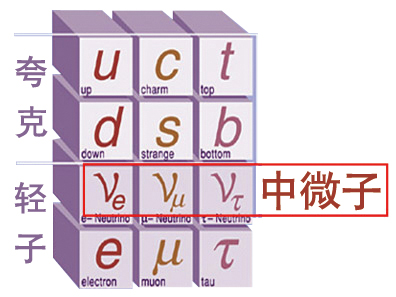
\includegraphics[height=5cm]{images/standarmodel.jpg}
 \caption{标准模型示意图}
 \label{fig:singleblock}
\end{figure}

中微子个头小,不带电,可自由穿过地球,与其他物质的相互作用十分微弱,号称宇宙间的"隐身人"。科学界从预言它的存在到发现它,用了20多年的时间。

目前标准模型中认为,3种中微子(电子中微子,$\nu$中微子和$\tau$中微子)是构成物质世界的最基本的十二种粒子之三,三种中微子味道中微子如下:

每一种中微子都对应一种带电的轻子——电子中微子对应电子,$\nu$中微子对应$\nu$子,同理,$\tau$中微子对应$\tau$子。

电子中微子:电子与原子相互作用,将能量一下子释放出来,会照亮一个接近球形的区域。

$\nu$中微子:$\nu$子不像电子那样擅长相互作用,它会在冰中穿行至少1千米,产生一个光锥。

$\tau$中微子:$\tau$子会迅速衰变,它的出现和消失会产生两个光球,被称为“双爆”。

\newpage
%----------------------------------SYSTEM DESIGN------------------------------------------
\subsection{中微子振荡}\label{sub:sysover}
中微子振荡(Neutrino oscillation)是一个量子力学现象,是指中微子在生成时所伴随的轻子(包括电子,$\nu$子和$\tau$子)味可在之后转化成不同的味,而被测量出改变。当中微子在空间中传播时,自发的会发生味道的周期性变化。

自然界中存在三种中微子,即电子中微子,μ中微子和τ中微子,分别对应了参与带电流弱相互作用的带电轻子。中微子振荡的验证了一种类型的中微子在传播一段距离后会变成另外一种类型的中微子。对这种现象的解释为三种中微子具有不同的静止质量且存在轻子混合态。换一种说法即是在传播过程中,中微子存在三种质量的本征态,分别对应了三个质量。如果存在轻子味道的混合,那么味道的本征态和质量的本征态就不会是一样的。当某弱相互作用产生中微子时,中微子的状态应该是三个量子本征态的叠加态,在传播的过程中,表现为质量本征态的相干叠加,当经过一段距离后,质量的本征态之间会产生一定的相位差,导致到达探测器中的中微子的状态和产生时的状态不一致。因此,可以将中微子振荡理解为具有本征态质量的中微子呈现出来的一种宏观相干叠加现象。
\begin{figure}[ht]
 \centering
 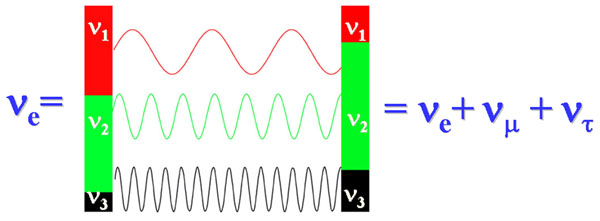
\includegraphics[height=5cm]{images/中微子振荡示意图.jpg}
 \caption{一个简单的中微子振荡图像表述}
 \label{fig:singleblock}
\end{figure}

接下来,本文将对中微子振荡进行一定的推导\footnote{引自:Neutrino Physics with JUNO}:
中微子的弱相互作用本征态可以写为:$\nu_{\alpha}$,其中,$\alpha=e,\mu,\tau$,而质量的本征态可以写为$\nu_{i}$,其中,$i=1,2,3$。
则态$\nu_{\alpha}$可以表示为质量态的叠加:
\begin{equation}
|\nu_{\alpha}>=\sum_{k}U_{\alpha k}^{*}|\nu_{k}>
\end{equation}
每个态的混合分量有因子$U_{\alpha k}^{*}$描述,这些因子可以从轻子混合矩阵所给出。
且本征态满足归一化条件和轻子混合的统一性:
\begin{equation}
\begin{split}
<\nu_{\alpha}|\nu_{\beta}>=\delta_{\alpha\beta}\\
<\nu_{i}|\nu_{j}>=\delta_{ij}
\end{split}
\end{equation}
质量的本征态满足Hamitonian方程:
\begin{equation}
H_{0}|\nu_{k}>=E_{k}|\nu_{k}>
\end{equation}
其中:$E_{k}^2=p^2+m_{k}^2$,p为中微子的动量,$m_{k}$为中微子的静止质量。
因此,薛定谔方程可以写为:
\begin{equation}
i\frac{\partial}{•\partial t}|\nu_{k}>=H_{0}|\nu_{k}>
\end{equation}
其解为:
\begin{equation}
|\nu_{k}(t)>=e^{-iE_{k}t}|\nu_{k}>
\end{equation}
带入到式(1):
\begin{equation}
|\nu_{\alpha}(t)>=\sum_{k}U_{\alpha k}^{*}|\nu_{k}(t)>=\sum_{k}U_{\alpha k}^{*}e^{-iE_{k}t}|\nu_{k}>
\end{equation}
做一个初始条件的约定:
\[|\nu_{k}>=|\nu_{k}(0)>\]
而式(1)的逆变换可以写为:
\begin{equation}
|\nu_{k}>=\sum_{k}U_{\alpha k}|\nu_{alpha}>
\end{equation}
带入到式(6)并用$\beta$代替$\alpha$:
\begin{equation}
|\nu_{k}(t)>=\sum_{\beta}U_{\beta k}^{*}e^{-iE_{k}t}|\nu_{\beta}>
\end{equation}
结合式(6)(8),可以得到:
\begin{equation}
|\nu_{\alpha}(t)>=\sum_{k,\alpha}U_{\alpha k}^{*}U_{\beta k}e^{-iE_{k}t}|\nu_{\beta}>
\end{equation}
由此,可以认为t时刻的中微子的态可以表示为初始时刻的本征态的叠加,


\newpage
\subsection{中微子的质量}\label{sub:sysover}
中微子振荡实验证明了中微子是有质量的,且存在味道的混合。在振荡实验中,已经精确的测量了两个独立的中微子质量平方差的值,当目前仍然对于三者的质量大小仍然是未知的。

同时,物理学界对于中微子的绝对质量也没有实际的观测,振荡实验只能得到质量的平方差值,对于具体的绝对质量是无法提供信息的。目前精确测量电子能谱,观测中微子质量带来的运动效应,最终得到的中微子的有效质量上限为\SI{2.2}{eV}(0.9的置信度)。

宇宙微波背景辐射和大尺度结构的观测,因为有质量的中微子会影响宇宙的演化。PLANCK实验组的最新观测结果显示三个中微子质量之和的上限为\SI{0.23}{eV}(0.95置信度),由此可以看出中微子的绝对质量不超过\SI{0.1}{eV}。然而,现在的实验数据仍不能排除最轻的中微子质量为零。(此部分的调研或推导未完成)

\newpage
\section{JUNO实验综述} \label{sysdes}%------------------------------

\subsection{JUNO中的中微子物理}\label{sub:sysover}
\subsubsection{中微子的质量顺序}\label{sub:sysover}
中微子振荡现象的发现确定了中微子的质量不为0,目前,标准的中微子的三味振荡的研究现状如下{\footnote{引自:Neutrino Physics with JUNO,p33}}:
\begin{itemize}
	\item{中微子MNSP轻子混合矩阵中三个非零混合角在精度在4\%到10\%得到了测量。}
    \item{中微子两个独立的质量平方差的大小已经测量,且测量精度优于4\%。}
    \item{目前测出的中微子质量平方差其中一个差得到的仅为其大小,对于其中的正负号仍然未知,因此,第三代中微子和前两代中微子的质量大小顺序是未知的。$\Delta m_{2,1}^2=m_{2}^2-m_{1}^2;|\Delta m_{3,1}^2|=|m_{3}^2-m_{1}^2|$}
    \item{混合角中的$\theta_{23}$只知道其范围,但不知其具体取值。}
    \item{轻子CP破坏中,在MNSP矩阵中的$\delta$ 未知。}
\end{itemize}

因此,测量中微子的质量顺序和CP破坏相角是未来一段时间内的重点。而JUNO实验的设计建设运行,将会给出对于中微子质量顺序的答案。

以下为JUNO实验测量中微子质量顺序(The neutrino mass hierarchy,简称MH)的原理{\footnote{引自:Neutrino Physics with JUNO,p33-38}}:

第三代中微子的质量和前面两代的质量相比,有两种可能的情况:第一种是认为第三代中微子的质量比第二代、第一代中微子的质量大(The normal mass hierarchy,简称NH);第二种则是认为第三代中微子的质量比前两代中微子的质量小(The Inverted mass hierarchy,简称IH)。
由中微子振荡的理论推导,可以得到\footnote{引自:\itshape{Neutrino oscillation phenomenology  in the standard model and beyond}  }:
 \begin{equation}
 \begin{split}
    \label{E1}
     P(\bar{\nu_e}-\bar{\nu_e},L)=1-{\sin^2{2\theta_{12}}} c_{13}^4\sin^2{\frac{\Delta{m_{21}^2}L}{4E}}-\\
\sin^2{2\theta_{13}} *[c_{12}^2\sin^2{\frac{\Delta{m_{31}^2}L}{4E}}+s_{12}^2\sin^2{\frac{\Delta{m_{32}^2}L}{4E}}]
 \end{split}
 \end{equation}

式(1)可写为:
 \begin{equation}
 \begin{split}
    \label{E1}
     P(\bar{\nu_e}-\bar{\nu_e},L)=1-\frac{1}{2}{\sin^2{2\theta_{13}}}[1-\sqrt{1-\sin^2{2\theta_{12}}}*\sin^2{\Delta_{21}}*\\\cos(2|\Delta_{ee}|\pm\phi)] -\cos^4{\theta_{13}}\sin^2{2\theta_{12}}\sin^2{\Delta_{21}} 
 \end{split}
 \end{equation}

其中:$\Delta_{ij}=\frac{\Delta{m_{ij}^2}L}{4E}$

$\Delta_{ee}=\Delta{m_{ee}^2}=\sin^2{\theta_{12}}\Delta{m_{31}^2}-\cos^2{\theta_{12}}\Delta{m_{32}^2}$

定义:$\Delta{m_{\phi}^2}=\frac{4E\phi}{L}$

则对于NH而言,中微子的质量平方差可以表示为:$2|\Delta{m_{ee}^2}|+\Delta{m_{\phi}^2}$,对于IH而言则可以表示为:$2|\Delta{m_{ee}^2}|-\Delta{m_{\phi}^2}$。这就使得NH和IH得到的振荡信号有所差异,这种差异在以L/E为谱的傅里叶变换中会表现得更加明显。

下图是反应堆中微子的傅立叶谱\footnote{引自:Neutrino Physics with JUNO,Fg2-5}:

\begin{figure}[ht]
 \centering
 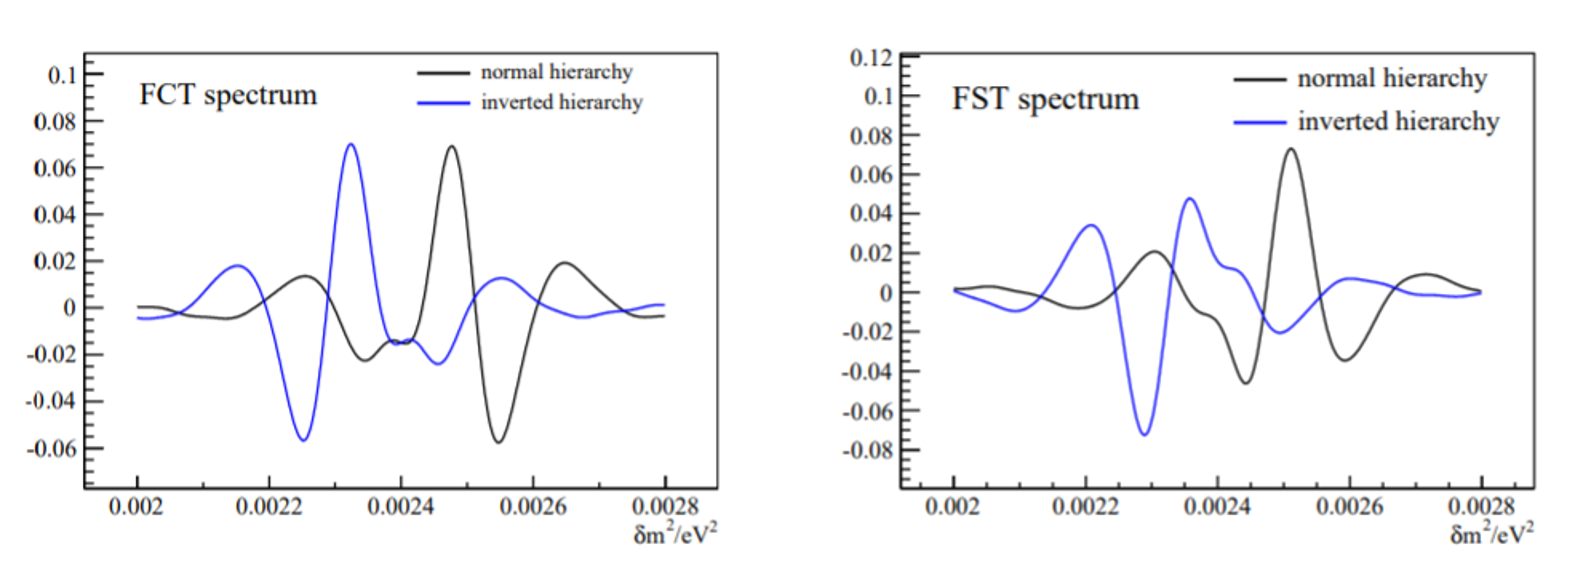
\includegraphics[height=5cm]{images/傅里叶图谱.png}
 \caption{反应堆反中子能谱的傅立叶余弦变换(FCT)(左面板)和傅立叶正弦变换(FST)(右面板)。黑线和蓝线分别代表NH和IH。}
 \label{fig:singleblock}
\end{figure}

从图中可以看到,IH和NH在余弦谱上都有有两个明显的峰,一个峰为正,一个峰为负,但是不同之处在于NH先出现正的峰,而IH先出现负的峰,且IH的两个峰的位置更加靠前。在正弦的谱上,则可以观察到IH有明显的负值峰,NH有一个明显的正值峰,且IH的峰出现在NH之前。因此,可以利用傅里叶谱区分出IH和NH,得到MH。

中距离的中微子实验测量$|\Delta{m_{ee}^2}|$,当与$|\Delta{m_{\mu\mu}^2}|$的测量结合时,可以得到更多关于MH的信息,这使得JUNO实验中,对于MH的测量显得更加的准确。

\subsubsection{JUNO 对中微子的精确测量}\label{sub:logicinter}

除了中微子的质量顺序问题,JUNO实验还将关注中微子振荡参数的精确测量以及测试三中微子标准模型。其具体的工作目标如下\footnote{引自:Neutrino Physics with JUNO,p54-55}:

\begin{itemize}
	\item{第一次同时观察由大气和太阳中微子质量平方差驱动的中微子振荡的实验。}
    \item{第一次对多振荡的大气中微子振荡进行观测。}
    \item{对中微子振荡参数:$\sin^2{\theta_{12}}$,$\Delta m^2_{21}$,$|\Delta m^2_{ee}|$进行高精度的测量,且测量精度优于1\%。}
\end{itemize}
*该部分的深入调研和推导还在进行中。

\subsubsection{JUNO其他相关中微子研究}

JUNO实验设备是目前世界上正在建设的最大的液闪探测器,优秀的分辨率和探测精度使得JUNO可以胜任很多的中微子研究。在太阳中微子研究、漫射超新星中微子背景、超新星中微子、大气中微子、地球中微子方面,都将在投入运行采数后发挥重要作用。

\subsection{实验方案}\label{sub:logicinter}

\subsubsection{JUNO的中微子信号}\label{sub:logicinter}

中微子是不带电的粒子,在实验上无法直接观测到,但是中微子会参与一些弱相互作用,产生特定的带电粒子,实验上通过观测中微子与物资作用后产生的次级粒子,可以间接的观测到中微子的信号。

JUNO是通过反$\beta$衰变(inverse beta decay,简称IBD)事件探测中微$$p+\bar{\nu}==e^{+}+n$$
当一个反中微子与质子作用后,会产生一个中子和一个正电子。正电子是空间中不稳定的存在,它会和物质中的电子发生湮灭过程,一个正电子和电子湮灭后会产生两个能量大小为0.511MeV的$\gamma$光子。

在衰变产生中子之后一段时间,中子会被氢原子核俘获,这个过程会在空间中激发光子,光子的能量大概是\SI{2.2}{MeV}。

如果探测器探测到这个中微子入射并与液闪作用,那么会在探测得到的波形中看到,在\SI{0.511}{MeV}处和\SI{2.2}{MeV}处形成两个峰。当然,这两个峰在时间上是有时间的先后顺序的,发生时间早的正电子湮灭过程会先在光谱上的\SI{0.511}{MeV}处形成观测峰,之后的200多ns后,释放\SI{2.2}{MeV}光子的过程也会完成,在信号的能量谱上形成\SI{2.2}{MeV}处的峰。这样就会形成两个在时间上有一定相关性的信号,可以通过做符合的方式来进行中微子的信号鉴别,取出中微子的信号。

\subsubsection{实验的探测器设计}\label{sub:logicinter}

江门中微子实验使用的是球体液闪探测器,装载着\SI{20}{kton}液体闪烁体的中心探测器放置在水池中,其建设结构如下图:\footnote{引自:Partical Identification at MeV energies in JUNO,Fg 1.}

\begin{figure}[ht]
 \centering
 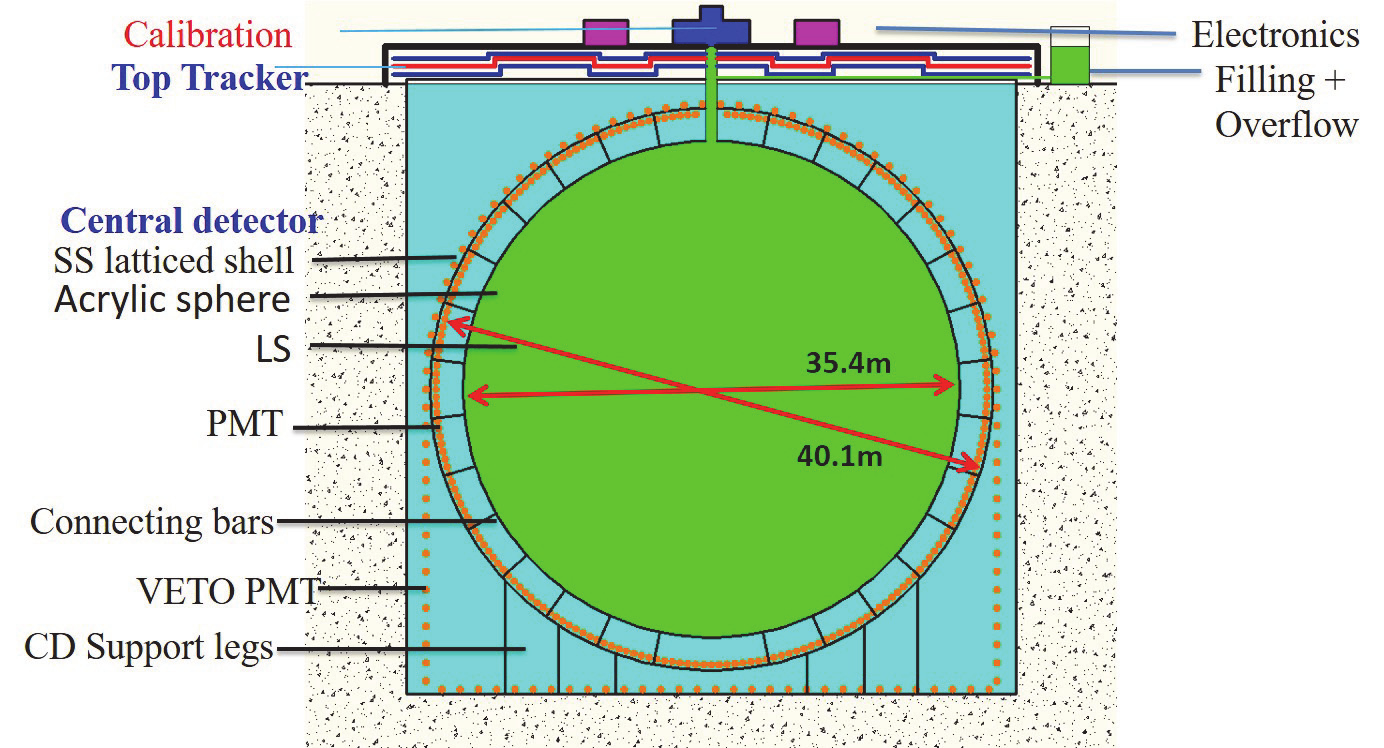
\includegraphics[height=7cm]{images/探测器示意图.png}
 \caption{液闪探测器示意图}
 \label{fig:singleblock}
\end{figure}

中心探测器的表面覆盖了4万多个光电倍增管,其中,18000个光电倍增管的直径为20英寸,分为13000个Micro-channel plates ( the Hamamatsu R12860 HQE )光电倍增管,用于传递和反射阴极射线来增加量子效率;5000个Dynode光电倍增管(NNVT),这是新型的双阴极管,具有很好的时间分辨率。25600个光电倍增管的直径为3英寸,均为HZC Photonics光电倍增管,将用作事件能量测定(双量热法)。这将有利于大型PMT系统的交叉校准,减少非线性,并将给检测器一个更大的动态范围和粒度\footnote{引自:Design and Status of JUNO ,p3}。

这些光电倍增管在经过测试后装备使用,在测试中,确定了电荷分辨率、单PE峰谷比、增益为$10^7$所需的工作电压、暗计数率(DCR)、单PE上升和下降时间以及预脉冲和后脉冲率。截至2019年7月已经测试的PMTs的PDE如图所示\footnote{引自:Design and Status of JUNO ,p3-4}。

\begin{figure}[ht]
 \centering
 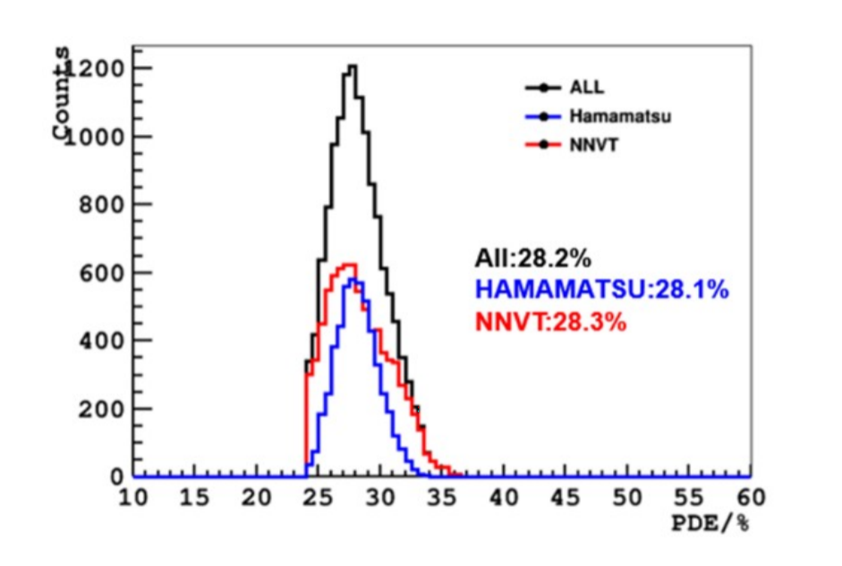
\includegraphics[height=7cm]{images/pmt测试.png}
 \caption{20英寸PMT的PDE测试结果,红色曲线为NNVT管,蓝色为Hamamatsu管,黑色为二者之和。}
 \label{fig:singleblock}
\end{figure}

探测器中装载了20kton的液体闪烁体介质,其中包含的成分为2.5g/L的PPO和1-4mg/L的bis-MSB,前者为产生光子的主要成分,后者能将光子的波长进行一定的移动,提高液闪探测器的透光率。

\subsubsection{JUNO的刻度系统}\label{sub:logicinter}
由信号的形成原理可以知道,JUNO实验是通过正电子的快信号和中子的慢信号做符合的方式来探测中微子的,为了满足实验的高精度及正常工作,则必须对实验探测器的能量响应和其随空间的变化做精确的标定,对探测器的标定内容通常需要包括:液闪的光学性质、探测器对中子的响应、探测效率以及俘获时间、探测器对于正电子响应、能量标度以及触发等。

JUNO实验有自己的一套刻度系统。主要包括了 Automatic Calibration Unit (ACU),
Cable Loop System (CLS),Guide Tube Control System(GTCS) and Remotely Operated under-liquidscintillator Vehicles (ROV)系统\footnote{这一部分未调研完各个刻度系统的具体作用}。

\subsubsection{JUNO TAO(台山反中微子观测台)}\label{sub:logicinter}

台山反中子观测台也是属于JUNO实验的一部分,使用的也是液体闪烁体探测器。

其目标在于精确测量反应堆中微子谱,为JUNO提供独立光谱参考;提供同位素产额和光谱,监控台山核反应堆;同时,它还要用于探测惰性中微子。

台山观测台使用的也是液体闪烁体探测器,其中心探测器是容纳26kton液体、直径为\SI{1.7}{m}的球体容器;液闪是掺入一定量的Gd的,工作温度控制在\SI{-50}{℃};表面光电倍增管的覆盖面积超过90\%,光子的探测率超过50\%。



\subsubsection{JUNO 优势及物理意义}\label{sub:logicinter}

JUNO实验主要依赖周围的核电站的中微子信号进行探测。在距离JUNO50多公里的地方,有阳江核电站和台山核电站,两个核电站功率达到了\SI{26.6}{GW},每天能探测到大概60个来自核反应堆的IBD事件。同时,JUNO对于其他来源的中微子也有足够的探测率:每天能探测到10-1000个太阳中微子,1-2个地球中微子,数个大气中微子。

在1-\SI{8 }{MeV}区间上,JUNO探测器的能量分辨率小于$\frac{3\%}{\sqrt{E}}$且能量探测的不确定度不到1\%,高精度的测量为解决中微子的质量排序问题提供了条件。

目前来说,JUNO实验设备正在建设中,其建设工作预计在2021年完成,投入使用。JUNO实验的开展,将进一步帮助科学家们了解微观粒子的相互作用。
\end{document}